\pagenumbering{arabic}
\section{Einleitung}
\label{s:intro}

Inhalt dieser wissenschaftlicher Arbeit ist das automatische Erstellen einer Material-Kostengliederung aus einer \ac{ifc}-Datei mit Hilfe von \ac{nlp} für eine Projekt einer Bausoftware. Diese Bausoftware ist die ORCA AVA aus dem mittelständigen Softwarehaus \glqq ORCA Software GmbH\grqq{} aus Neubeuern. 
In diesem Kapitel soll eine kurze Einführung über die \glqq ORCA Software GmbH\grqq{} und das Produkt  ORCA AVA gegeben werden. Außerdem wird die Motivation für das Feature und die wissenschaftliche Vorgehensweise dieser Arbeit beschrieben.

\subsection{Ausgangssituation}
\label{c:intro:start}

Die im Titel beschriebene Bausoftware ist die ORCA AVA aus dem Softwarehaus \glqq ORCA Software GmbH\grqq{}. Dieses wurde im Jahr 1990 von Dipl.-Ing. Siegfried Tille und Dipl.-Ing. Heinz Nießen gegründet. Der Hauptsitz des Unternehmens ist in Neubeuern, bei Rosenheim. Das Unternehmen ist auf die Produktentwicklung von Software für die Baubranche spezialisiert. Im Vordergrund stehen die Ausschreibungssoftware ORCA AVA und die Ausschreibungstext-Plattform AUSSCHREIBEN.DE. Ziel der Entwicklung ist es die \ac{ava} eines Bauvorhabens für Planer, Architekten und Bauingenieure zu vereinfachen. Der Leitfaden ist, dass die Software soll für jeden verständlich und intuitiv zu bedienen sein.
Diese Arbeit fokussiert sich auf eine Erweiterung der ORCA AVA. Sie ist für alle Architektur- und
Ingenieurbüros, Wohnungsbaugesellschaften, Unternehmen und Behörden zur einfachen Abwicklung von Bauprojekten mit Ausschreibung, Vergabe und Abrechnung. Zusätzlich bildet sie das Kostenmanagement von solchen Projekten ab. Die Software ist außerdem \ac{bim} fähig und bietet \ac{din} zertifizierte Schnittstellen für den Datenaustausch an. Es stehen drei verschiedene Editionen zur Verfügung. Die ORCA AVA \ac{se}, die ORCA AVA \ac{pe} und die ORCA AVA \ac{ee}.  Die aktuellste Version ist die 25.0.

Technisch wird die ORCA AVA in .NET entwickelt. Ein Großteil der Anwendung besteht noch aus \ac{vb} Code. Alle neuen Komponenten und Erweiterungen werden in C\# implementiert. Neue \ac{gui}-Komponenten werden dementsprechend mit \ac{wpf} entwickelt. \ac{wpf} ist ein .NET Framework für das Erstellen von Windows Applikationen mit graphischer Benutzeroberfläche von Microsoft. \citep{Microsoft_2022} Die ORCA AVA und der IFC Manager (siehe Abschnitt \ref{s:basics:ifc:usage}) laufen in eigenen Prozessen und kommunizieren auf Prozessebene in der lokalen Umgebung. 

\subsection{Motivation}
\label{c:intro:motivation}

Ziel ist es \ac{bim} noch mehr in die ORCA AVA zu integrieren. \ac{bim} bedeutet, dass die Planung von Bauprojekten vollständig auf digitaler Basis durchgeführt wird.  Für jeden Projektbeteiligten besteht somit jederzeit Zugriff auf alle projektrelevanten Daten über Kosten, Mengen und Zeitabläufen. Somit können Baukosten einfacher ermittelt und der Bauprozess besser überwacht werden. In Abbildung\,\ref{fig:bim} ist zu sehen, dass \ac{bim} ein Relevanter Begriff in der Baubranche ist. Die Verwendung der Praktik ist allerdings noch nicht sehr verbreitet \citep[p.~20]{Thomas_Baumanns_Dr_Philipp-Stephan_Freber_Dr_Kai-Stefan_Schober_Dr_Florian_Kirchner2016-gu}. Mit dem \glqq \ac{ifc} First\grqq{} Ansatz ist das langfristige Ziel der ORCA AVA das Thema \ac{bim} noch mehr abzudecken. Aus den Daten des 3D-Gebäudemodells soll automatisch ein Ausschreibungstext entstehen. Bauteile aus dem Gebäudemodell sollen mit Kurztext, Langtext, Menge, Preis und vordefinierten Kostengliederungen in den Programmteil Bauelemente der ORCA AVA übernommen werden. Das ganze ist ein gutes Werbemittel für den Verkauf der Software, da die Relevanz des Themas so hoch ist und somit viele Kunden anspricht. Ein erster Teil des langfristigen Ziels, ist die Übernahme der Baustoffe aus der \ac{ifc}-Datei. Diese bieten die erste Kostengliederung für den \glqq \ac{ifc} First\grqq{} Ansatz. Die Übernahme von weiteren Daten aus dem \ac{ifc}-Modell können darauf aufgebaut werden.
\begin{figure}[h]
	\centering
	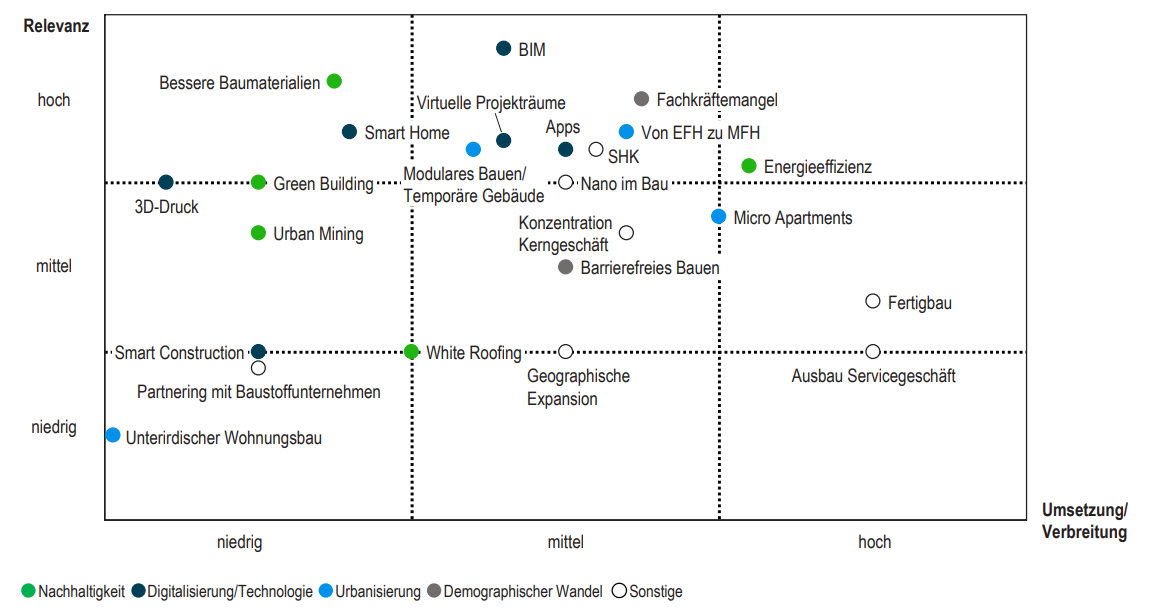
\includegraphics[scale=0.52]{bim-relevanz}
	\caption[Relevanz \ac{bim}]
	{Megatrends Nachhaltigkeit und Digitalisierung in der Bauwirtschaft. Bilder aus \citep[p.~20]{Thomas_Baumanns_Dr_Philipp-Stephan_Freber_Dr_Kai-Stefan_Schober_Dr_Florian_Kirchner2016-gu}}
	\label{fig:bim}
\end{figure}
Ein weiterer Trendbegriff, der mit dem Feature abgedeckt werden soll ist \glqq Künstliche Intelligenz\grqq{} und \glqq Maschinelles Lernen\grqq{}. Das Suchinteresse der beiden Themen sind in Abbildung\,\ref{fig:ki-ml-trend} zu sehen. Die Werte geben das Suchinteresse relativ zum höchsten Punkt im Diagramm an. Der Begriff \glqq Maschinelles Lernen\grqq{} hat seit Anfang 2015 eine steigendes Suchinteresse. Bei \glqq künstliche Intelligenz\grqq{} ist das Suchinteresse von Anfang 2017 bis Ende 2021 konstant hoch. Der starke Anstieg ab November 2022 hängt wahrscheinlich mit der Veröffentlichung der Software ChatGPT zusammen. Man erkennt insgesamt, dass das Interesse über die letzten Jahre ist. Diese Begriffe werden von der vertrieblicher Seite schon länger gewünscht. Die Erweiterung wäre der erste Einsatz von Maschinellem Lernen. Es ist also zusätzlich auch ein Pilotprojekt, um Erfahrungen in diesem Themengebiet zu bekommen. Außerdem lernt die Entwicklung das Arbeiten mit solchen Algorithmen.

Durch die genannten Punkte ist das Feature dem Kano-Modell nach als Begeisterungsfeature zuzuordnen. Die Kundenzufriedenheit steigt also exponentiell mit dem Erfüllungsgrad der Anforderung. (siehe Abbildung\,\ref{fig:kano-model}) Mit der Zeit wandelt sich es dann erst in ein Leistungsfeature und irgendwann in ein Basisfeature. \citep[p.~3-4]{Hölzing_2008}

\begin{figure}[h]
	\centering
	
	\begin{subfigure}{0.99\textwidth}
		\centering
	\includegraphics[width=1\linewidth]{künstiliche-intilligenz-trend}
		\caption{Suchinteresse: Künstliche Intelligenz}
		\label{FIG:ki-trend}
	\end{subfigure}
	\hspace{1cm}
	\begin{subfigure}{0.99\textwidth}
		\centering
	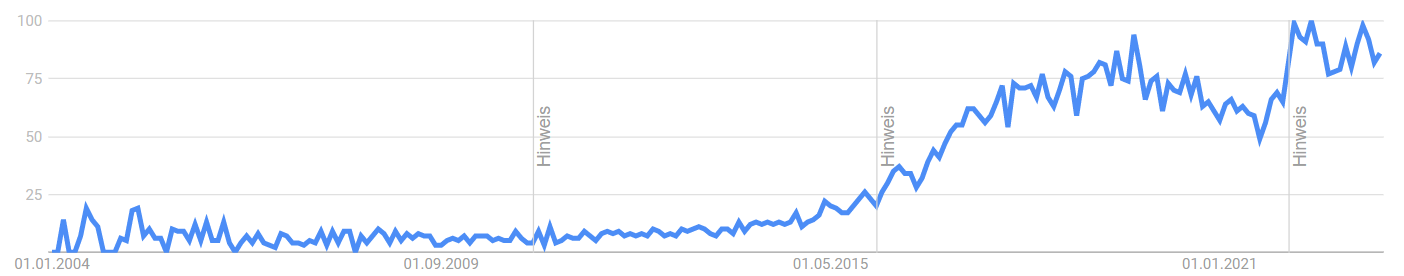
\includegraphics[width=1\linewidth]{machine-learning-trend}
		\caption{Suchinteresse: Machine Learning}
		\label{FIG:ml-trend}
	\end{subfigure}
	
	\caption[Google Trends]{Google Suchinteresse der beiden Begriffe \glqq künstliche Intelligenz\grqq{} und \glqq Maschinelles Lernen{} seit 2004}
	\label{fig:ki-ml-trend}
\end{figure}

\begin{figure}[h]
	\centering
	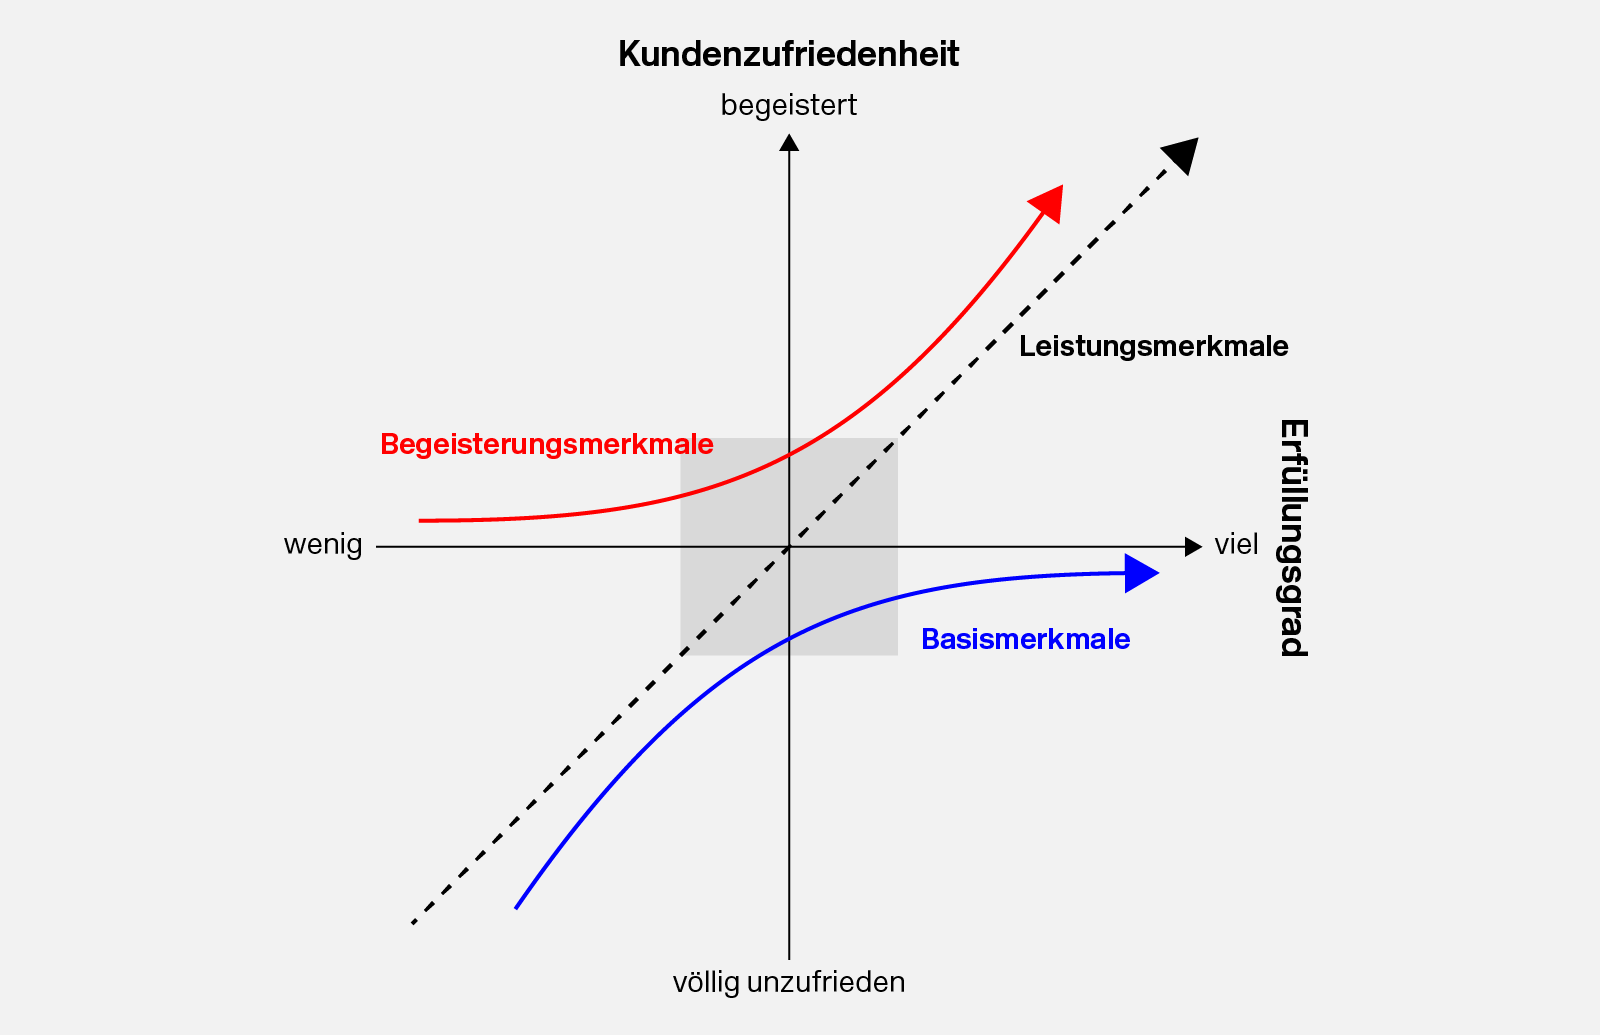
\includegraphics[width=1\linewidth]{kano-modell}
	\quelle{https://dmexco-lightsails-media.s3.eu-central-1.amazonaws.com/wp-content/uploads/2021/01/04112832/Kano-Modell.png (Accessed: 2023-2-24) }
	\caption[Kano Modells]{Kano Modell der Kundenzufriedenheit}
	\label{fig:kano-model}
\end{figure}

\subsection{Ziel der Arbeit}
\label{c:intro:target}



\subsection{Wissenschaftliche Vorgehensweise}
\label{c:intro:methodology:scientific_proceture}
Im Folgenden wird die wissenschaftliche Vorgehensweise der Arbeit aufgezeigt.
In Abschnitt \ref{s:intro} wurde bereits die Ausgangssituation beschrieben und das entwickeln des Features motiviert. Außerdem wurde das Ziel der Arbeit definiert. Im nächsten Kapitel, Kapitel\,\ref{s:basics}, werden Grundlagen erläutert, auf die diese Arbeit aufbaut. Im anschließenden Kapitel\,\ref{s:requirements} sollen die Problemstellung und Anforderungen analysiert werden. %todo 

\newpage
\section{Grundlagen}
\label{s:basics}
In diesem Kapitel werden die Grundlagen im Bereich der Fachspezifischen Themen, Technik und Projektmanagement vermittelt. Dies sollte Verständnis für die folgenden Kapitel schaffen. Zuerst geht es um das Projektmanagement. Anschließend geht es um das Format \ac{ifc}, dessen Geschichte und dessen Nutzungsmöglichkeiten für diese Arbeit. Außerdem wird die Struktur und der Nutzen einer Kostengliederung in der ORCA AVA veranschaulicht.

\subsection{Projektmanagement}
\label{s:basics:project-management}
Bevor auf technische und fachliche Aspekte von \ac{ifc} und Kostengliederungen eingegangen wird, folgt die Einführung in das Projektmanagements mit SCRUM und \ac{devops}.

\subsubsection{Vorgehensmodell}
\label{s:basics:project-management:procedure_model}
Das Projekt wurde mit Hilfe agiler Softwareentwicklung durchgeführt. Die durchlaufenden Sprints sind zwei Wochen lang. Funktionale Anforderungen werden vom Projektmanagement gestellt.

\subsubsection{DevOps}
\label{s:basics:project-management:devops}
Die Bezeichnung \ac{devops} vereint die beiden Praktiken \glqq Development\grqq{}(Entwicklung) und \glqq Operations\grqq{}(Vorgänge). Die traditionelle Trennung von Entwicklung und Softwarebetrieb führt oft zu
Interessenskonflikten. Entwickler wollen stetig die Software verbessern, der Betrieb will Änderungen vermeinden um die Stabilität des Systems zu gewährleisten. Durch \ac{devops} entsteht ein Softwareentwicklungsprozess, den man durch Praktiken wie Continous Integration, Continous Delivery, Continous Deployment, automatisiertes Teste, Infrastructure-as-Code und automatische Veröffentlichungen beschleunigt. DevOps steht auch für eine Entwicklungskultur mit offener Zusammenarbeit, Kommunikation, Transparenz und Eingestehen von Fehlern, um Konflikte im Team zu vermeiden. Im Entwicklungsteam der ORCA AVA wird diese Praktik umgesetzt.
Die Technischen Hilfsmittel, die für den DevOps Prozess verwendet werden, sind in Abschnitt \ref{s:qs:technical_aids} \citep{devops_2021}

\subsection{\ac{ifc}}
\label{s:basics:ifc}
Die Daten für die Material-Kostengliederung werden aus einem digitalem Gebäudemodel entnommen. Der öffentliche internationale Standard (ISO 16739-1:2018) für Gebäudemodelle ist \ac{ifc}. \citep{BuildingSMART_International_Ltd2017-gs} Dieser wird auch in der bestehenden ORCA AVA benutzt um den Ausschreibungsprozess zu unterstützen. IFC Dateien können geöffnet, angeschaut und Informationen über das Modell in die Hauptsoftware übernommen werden. Im folgenden Kapitel wird die Geschichte, das Format von \ac{ifc} und die Verwendung in der ORCA AVA erläutert.

\subsubsection{Geschichte}
\label{s:basics:ifc:history}
\ac{ifc} ist die Hauptleistung der buildingSMART International, Ltd.  Die non-profit Organisation will mit der Spezifikation den BIM Prozess fördern und voranbringen. \citep{BuildingSMART_IFC}
Angefangen hat die Organisation als der Verein Industrieallianz für Interoperabilität IAI e. V. mit Sitz in Berlin. 1994 startete die Entwicklung an dem offenen Datenmodellstandard \ac{ifc}. Dieser sollte die Anforderungen der Industrie an Interoperabilität gerecht werden und eine gemeinsame Basis zum Austausch von Informationen durch verschiedenen Anwendungen geschaffen werden. Im Zusammenhang mit \ac{bim} sollten Daten lesbar, editierbar für verschiedene Systeme durch den Bauprozess und kompletten Lebenszyklus eines Gebäudes geteilt werden. \citep{Laakso2012-oi} Nach einigen Prototypen wurde 1999 \ac{ifc} 2.0 veröffentlicht. Diese wurde bis 2007 mit der Version 2.3.0.1 steig verbessert. Die Version 2.3 wird auch in heutigen Projekten noch verwendet. 2013 wurde \ac{ifc}4 veröffentlicht, welche mit der Version 4.0.2.1 die aktuellste, offizielle IFC Version ist. Das Format wird aktuell noch stetig weiterentwickelt. Neue Versionen stehen schon vor einer Abstimmung der \ac{iso}. \citep{BuildingSMART_history_2022} Es gibt folgendermaßen aktuell zwei offizielle Versionen. Beide werden in der Praxis benutzt und wie in Abschnitt \ref{s:basics:ifc:usage} beschrieben mit der ORCA AVA kompatibel.


\subsubsection{Format}
\label{s:basics:ifc:format}
Das \ac{ifc} Format kodiert folgende Daten:
\begin{itemize}
	\item Identität, Semantik, Attribute und Relationen von Objekten
	\item Abstrakte Konzepte wie Performance oder Kosten
	\item Prozesse wie z.B.Installationen und Operationen
	\item Personen wie z.B. Eigentümer oder Lieferanten
\end{itemize}
Die Spezifikation kann also für das Bauen, Betreiben oder Nutzen eines Gebäudes genutzt werden. IFC ist ein Implementierungs- Unabhängiges Datenmodell, welches in verschiedenen Umgebungen und elektronischen Formaten benutzt werden kann. Es kann beispielsweise in eine relationales Datenbankschema gegossen oder auch als Dateiformat implementiert werden. Das weitverbreiteste Format ist \ac{spf} \citep{Laakso2012-oi,BuildingSMART_IFC}. Das \ac{step} ist das kompakteste Format für den dateibasierten Import und Export von \ac{ifc}-Dateien. Des weiteren kann es als \ac{xml} oder ZIP Datei verwendet werden. \citep{BuildingSMART_IFC}


\subsubsection{Verwendung}
\label{s:basics:ifc:usage}
\begin{displayquote}
	Today, \ac{ifc} is typically used to exchange information from one party to another for a specific business transaction. \citep{BuildingSMART_IFC}
\end{displayquote}
In der ORCA AVA wird \ac{ifc} für das Einlesen und Übernehmen von Maßen und Mengen in die Ausschreibung verwendet. Es vereinfacht den Prozess, die in der \ac{cad}-Software erstellten Daten einfach in die Leistungsverzeichnisse der ORCA AVA zu überführen.
Die ORCA AVA kann \ac{ifc}-Dateien einlesen. Im \ac{ifc} Manager wird das 3D-Modell dann angezeigt. In dem geöffneten Fenster gibt es einige fachliche Ansichten, die jegliche \ac{ifc}-Daten nochmal fachlich abstrahieren. In den Ansichten können zum Beispiel bestimmte Maße oder die Anzahl verschiedener Bauteile, die aus dem \ac{ifc}-Modell berechnet werden, in die ORCA AVA übernommen werden.
Es werden auch alle im \ac{ifc} definierten Eigenschaften eines Bauteils in der Eigenschaften-Ansicht angezeigt. Hier kann man auch die Materialbezeichnung des Bauteils finden, die im Modell hinterlegt ist. In Abbildung\,\ref{fig:ifc-manager} ist die Oberfläche des \ac{ifc} Managers zu sehen. Man sieht die Materialangabe rechts unten im Eigenschaftenfeld unter dem 3D-Modell.

Für das Arbeiten mit \ac{ifc}-Dateien wird die open-source Bibliothek xbim-toolkit verwendet. Die .NET Bibliothek kann \ac{ifc}-Dateien lesen, schreiben und anzeigen. Außerdem unterstützt es bei der Berechnung von komplexer Geometrie, um die Modelldaten für Analysen nutzbar zu machen. Seit 2009 wird die Bibliothek in Zusammenarbeit mit der Norhumbria Untiversity weiterentwickelt. Mittlerweile bildet es die Standards \ac{ifc2x3} und \ac{ifc4} zu 100\% ab. Außerdem bietet es an, auch \ac{ifc2x3} Modelle über das IFC4 Interface anzuprogrammieren. Somit können mit einer Codebasis beide Formate abgebildet und unterstützt werden. \citep{Xbim_ltd_undated-wm}


\subsubsection{Möglichkeiten für die  Materialangabe eines Bauteils}
\label{s:basics:ifc:buildingmaterial}
In einem \ac{ifc}-Modell können Materialien unterschiedlich einem Bauteil zugewiesen sein. Die Spezifikation bietet die Klasse \textit{IfcMaterial}. Diese bildet fachlich ein Material ab. Es hat die Attribute Name, Description und Category.\citep{ifc_material} Eine Instanz von \textit{IfcMaterial} kann mit einem Element oder Elementtyp über die \textit{IfcRelAssociatesMaterial} verbunden werden. Diese Zuweisung kann über verschiedene Weisen stattfinden. In Abbildung \ref{fig:material-single} ist eine direkte Zuweisung über das \textit{IfcRefAssociatesMaterial} zu sehen. Hier hängt das \textit{IfcMaterial} direkt am Element. 
Bei einer Platte mit mehreren Schichten kann das \textit{IfcMaterial} auch wie in Abbildung \ref{fig:layer-set} zu sehen an einem \textit{IfcMaterialLayerSet} zugewiesen sein. Jede Schicht hat hier seine eigne Dicke und eigene Materialangabe. 
Ein Träger kann das \textit{IfcMaterial} über ein \textit{IfcMaterialProfileSet} abgebildet haben. (siehe Abbildung \ref{fig:profile-set})
Bei zum Beispiel einer Tür können verschiedene Materialien des Rahmens und der Verglasung über das \textit{IfcMaterialConstituentSet} abgebildet werden. (siehe Abbildung \ref{fig:constituent-set}) \citep{ifc_material_association}
Zusätzlich gibt es noch ältere Möglichkeiten Materialangaben an ein Element zu binden. In \ac{ifc2x3} gibt es die Klasse \textit{IfcMaterialList} \citep{Thomas2007_MaterialList}. Diese Möglichkeit ist deprecated, in der Praxis kommt das \ac{ifc2x3} Format noch regelmäßig vor. Die \textit{IfcMaterialList} muss also auch beachtet werden.

Neben verschiedenen Verbindungen zu \textit{IfcMaterial} hat jedes Element bei \ac{ifc} auch verschiedene Property Sets. Property Sets sind Container, die Eigentschaften je nach ihrem Namensattribut enthalten. Einige Propertiy Sets sind in der Spezifikation des \ac{ifc} Standards enthalten. Es können auch zusätzlich benutzerdefinierte Property Sets erfasst werden. Diese können auch Informationen über das Material eines Elements enthalten. \citep{ifc_property_set} Das PropertySet \textit{Pset\_MaterialConcrete} weißt darauf hin, das es sich um Beton handelt.

\begin{figure}[h]
	\centering
	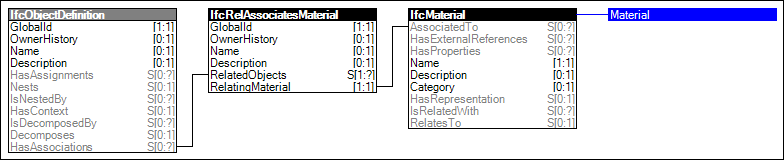
\includegraphics[width=1\linewidth]{material-single}
	\caption[IfcMaterial]{Material Single Association}
	\label{fig:material-single}
\end{figure}

\subsection{Das Format Kostengliederung in der ORCA AVA}
\label{s:basics:coststructure}
Die Kostengliederung bietet eine Struktur, um Gesamtkosten einer Baumaßnahme in Kostengruppen unterteilt auswerten zu können. Logisch zusammengehörende Kosten können so in eine \ac{kg} zusammengerechnet werden. Außerdem ist der Aufbau eine Baumstruktur, wodurch Kostengruppen hierarchisch addiert werden können. 
Bei einem Bauprojekt kann man so Kosten über alle Projektphasen vergleichen. Von der Kostenschätzung über die  Ausschreibung bis zur Rechnungsfreigabe. So können Kostenauswertungen nach den verschiedenen Kostengruppen durchgeführt werden. In einem ORCA AVA Projekt kann man verschiedene Kostengliederungen definieren. Es existieren bereits Standardkostengliederungen beim Erstellen eines neuen Projektes. Zusätzlich können neue Kostengliederungen erstellt oder importiert werden.\citep{noauthor_undated-bx}


Technisch ist eine Kostengliederung als Modell im C\# Code definiert. Der Aufbau bildet die Baumstruktur über eine Referenz zur ParentNode und mehreren ChildrenNodes ab. Das Model kann über die ORCA AVA interne Middleware in der Datenbank persistiert werden. Die persistierten Kostengliederungen werden dann über VB-Teil der Anwendung im entsprechenden Programmteil angezeigt.
So müssen nach der generierten Kostengliederungs-Struktur die strukturierten Materialbezeichnungen in das C\# Modell abgebildet werden. So wird nach dem Import die erstellte Kostengliederung automatisch in der Oberfläche angezeigt und kann für Kostenauswertungen benutzt werden.

\newpage
\section{Problemstellung und Anforderungen}
\label{s:requirements}
\subsection{Problemstellung}
\label{s:requirements:problem}
\subsection{Anforderungen}
\label{s:requirements:requirements}
\subsubsection{Funktionale Anforderungen}
\label{s:requirements:requirements:functional}
\subsubsection{Weitere Anforderungen}
\label{s:requirements:requirements:additional}
\subsubsection{Ziele}
\label{s:requirements:requirements:goals}

\newpage
\section{Theoretische Konzeption für die Erstellung der Material-Kostengliederung}
\subsection{{Textklassifizierungsalgorithmus \dots}}
\subsection{{WordNet \dots}}
\subsection{\dots}

\newpage
\section{Gegenüberstellung der möglichen Konzepte}
\subsection{Messkriterien}
\subsection{Vergleich der Konzepte}
\subsection{Festsetzten eines Algorithmus}

\newpage
\section{Praktische Umsetzung}
\subsection{Zusammenfassen der Materialschnittstelle einer IFC Datei}
\subsubsection{Entwurf des Algorithmus}
\subsubsection{Implementieren des Algorithmus}

\subsection{Standardisierung der Materialnamen}
\subsubsection{Nutzen von Artificial Inteligence}

\subsubsection{Erstellen einer Datengrundlage}
\subsubsection{Implementierung der Standardisierung}

\subsection{Erstellen einer Kostengliederung}
\subsubsection{Implementieren}

\newpage
\section{Maßnahmen zur Qualitätssicherung}
\label{s:qs}
\subsection{Clean Code}
\label{s:qs:cleancode}
\subsection{Technische Hilfsmittel}
\label{s:qs:technical_aids}
\subsection{Tests und Abnahme}
\label{s:qs:tests}

\newpage
\section{Abschluss}
\label{s:closing}
\subsection{Bewertung der praktischen Umsetzung}
\label{s:closing:rating}
\subsection{Fazit}
\label{s:closing:conclusion}
\subsection{Ausblick}
\label{s:closing:outlook}
 Jo viel Spaß noch
